\documentclass[a4paper,12pt]{article}
\usepackage{amssymb}
\usepackage{graphicx}
\usepackage{amsmath}
\graphicspath{{fig/}}
\begin{document}

\title{CVTree \\\Large{(Standalone Version)}\\User's Manual}
\author{Guanghong Zuo and Bailin HAO}
\date{\today}
\maketitle

%\newpage

CVTree stands for {\bf Composition Vector Tree} which is the
implementation of an alignment-free algorithm to generate a
dissimilarity matrix from comparatively large collection of DNA or Amino
Acid sequences, preferably whole-genome data, for phylogenetic studies.

There are two versions of the program:
\begin{enumerate}\itemsep 0pt
\item {\bf CVTree Web Server} which has been published twice in the Web
  Server Issues of {\it Nucleic Acids Research}, \cite{qlh04}
  and\\ \cite{xh09}. The lastest CVTree Web Server, CVTree3 Web Server \cite{zh15}, have two identical but independent installations:
  \begin{itemize}
  	\item Fudan University, Shanghai: \\
  	  {\tt http://tlife.fudan.edu.cn/cvtree/} 
  	\item Beijing Institute of Genomics, Beijing:\\
    {\tt http://cvtree.net 
    \\ http://bigd.big.ac.cn/cvtree} 
  \end{itemize}

\item {\bf CVTree Standalone Version} which is provided to those who are
  interested in the intermediate results, e.g., the collection of all
  CVs, or deal with extremely huge datasets of their own. We provide
  also a few options and scripts that were not available in the Web
  Server versions. 
\end{enumerate}


\section{The Installation}
\subsection{Preparation}
\begin{itemize}
	\item cmake $\geq$ 2.8.4
  \item g++ $\geq$ 4.8 or other compiler supporting C++11 standard
  \item compiler with support openmp for parallel
	\item Library: libz, netcdf, netcdf\_cpp
\end{itemize}

\subsection{Compiling}
Unzip or checkout the source files, Obtained the compiling option by
cmake
\begin{itemize}
	\item unzip the package file and change into it
	\item mkdir build and change into it
	\item cmake .. or add some options you wanted, e.g.:\\ -DCMAKE\_INSTALL\_PREFIX=/usr/local
  \item make
  \item make manual
	\item make install
\end{itemize}

\section{Programs and Command-Line Options}
All the programs was implemented in C++.

\subsection{cvtree: the all in one command}
\subsubsection{The Flow of cvtree command}
The cvtree command is the main command for the software. It generate the the phylogeny tree 
from the fasta files directly. 

\begin{figure}[!h]
  \centering
  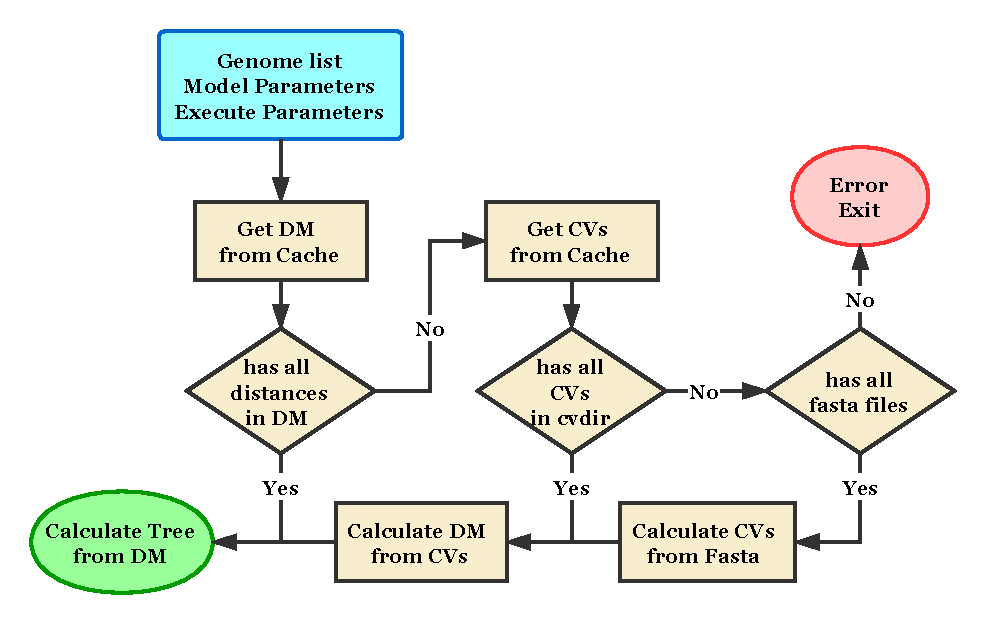
\includegraphics[width=0.8\textwidth]{Flowchart.pdf}
  \caption{The Flowchart of the cvtree command}
\end{figure}

\subsubsection{The command usage}
\begin{itemize}\itemsep 0pt
  \item cvtree -- Generate nwk tree from input genomes
\begin{verbatim}
  cvtree
  [ -d <dm> ]         Output distance matrix format, defaut: <Method><Suffix><K>
  [ -t <nwk> ]         Output distance matrix format, defaut: <Method><Suffix><K>.nwk
  [ -G <dir> ]        Input genome file directory
  [ -g faa ]          the type of genome file, defaut: faa
  [ -V <cvdir> ]      Super directory of cv files
  [ -i list ]         Genome list for distance matrix, defaut: list
  [ -k '3 4 5 6 7' ]  values of k, defaut: N = 3 4 5 6 7
  [ -r <matrix> ]     Reference distance matrixs, splite with ','
  [ -M <N> ]          Runing memory size as G roughly,
                      default 80% of physical memory
  [ -m Hao/InterList/InterSet]    Method for cvtree, defaut: Hao
  [ -C ]              Force use the netcdf compress distance matrix
  [ -q ]              Run command in queit mode
  [ -h ]              Disply this information
\end{verbatim}
\end{itemize}



\subsection{Obtain Phylogeny Tree Step by Step}
\begin{itemize}\itemsep 0pt
  \item cv -- Generate CV files from input data
\begin{verbatim}
cv [ -G <dir> ]        input genome file directory
[ -V <dir> ]        output cv directory
[ -i list ]         input species list, defaut: list
[ -f <Fasta> ]      get cv for only one fasta
[ -k '3 4 5 6 7' ]  values of k, defaut: N = 3 4 5 6 7
[ -g faa ]          the type of genome file, defaut: faa
[ -m Hao/InterList/InterSet]    the method for cvtree, defaut: Hao
[ -q ]              Run command in queit mode
[ -h ]              disply this information
\end{verbatim}

  \item dist -- Generate distance matrix based on CV files
\begin{verbatim}
  dist
  [ -o <dm> ]      Output distance matrix, defaut: <Method><Suffix>
  [ -V <cvdir> ]   Super directory of extend cv files
  [ -i list ]      Genome list for distance matrix, defaut: list
  [ -s <Suffix> ]  Suffix of the cvfile, default: .faa.cv6
  [ -r <matrix> ]  Reference distance matrixs, splite with ','
  [ -M <N> ]       Runing memory size as G roughly,
                   default 80% of physical memory
  [ -m Hao/InterSet/InterList] Method for cvtree, defaut: Hao
  [ -C ]           Force use the netcdf compress distance matrix
  [ -q ]           Run command in queit mode
  [ -h ]           Disply this information
\end{verbatim}

\item nj -- Generate newick tree from distance matrix by using the Neighbor-Joint method
\begin{verbatim}
  nj
  [ -d infile ]     Input distance matrix, defaut: dist.matrix
  [ -o Tree.nwk ]   Output newick tree, defaut: Tree.nwk
  [ -i <list> ]     selection index list of the distance matrix,
                    if no defined, whole distance matrix are used
  [ -C ]            Use the netcdf input format, default false
  [ -q ]            Run command in queit mode
  [ -h ]            Disply this information
\end{verbatim}
\end{itemize}

\subsection{Tools}
\begin{itemize}
  \item cvdump -- convect the binary cv file to acsii file
\begin{verbatim}
cvdump  -i <cvfile>        input file name
 [ -g faa|ffn ]      the type of genome file, defaut: faa
 [ -n ]              output the number code, default: the letters
 [ -h ]              disply this information
\end{verbatim}

\item getdist -- get the distance from distance matrix
\begin{verbatim}
  getdist [ -d infile ]       distance matrix files list separate by :, default: infile
  [ -i selfile ]      the select genomes, defaut: none
  [ -H ]              whether output html table, default: false
  [ -l ]              get the list of species of distance matrix
  [ -h ]              disply this information
\end{verbatim}
\end{itemize}

\section{The Algorithm}
\subsection{CVTree scheme}
\begin{figure}[!h]
  \centering
  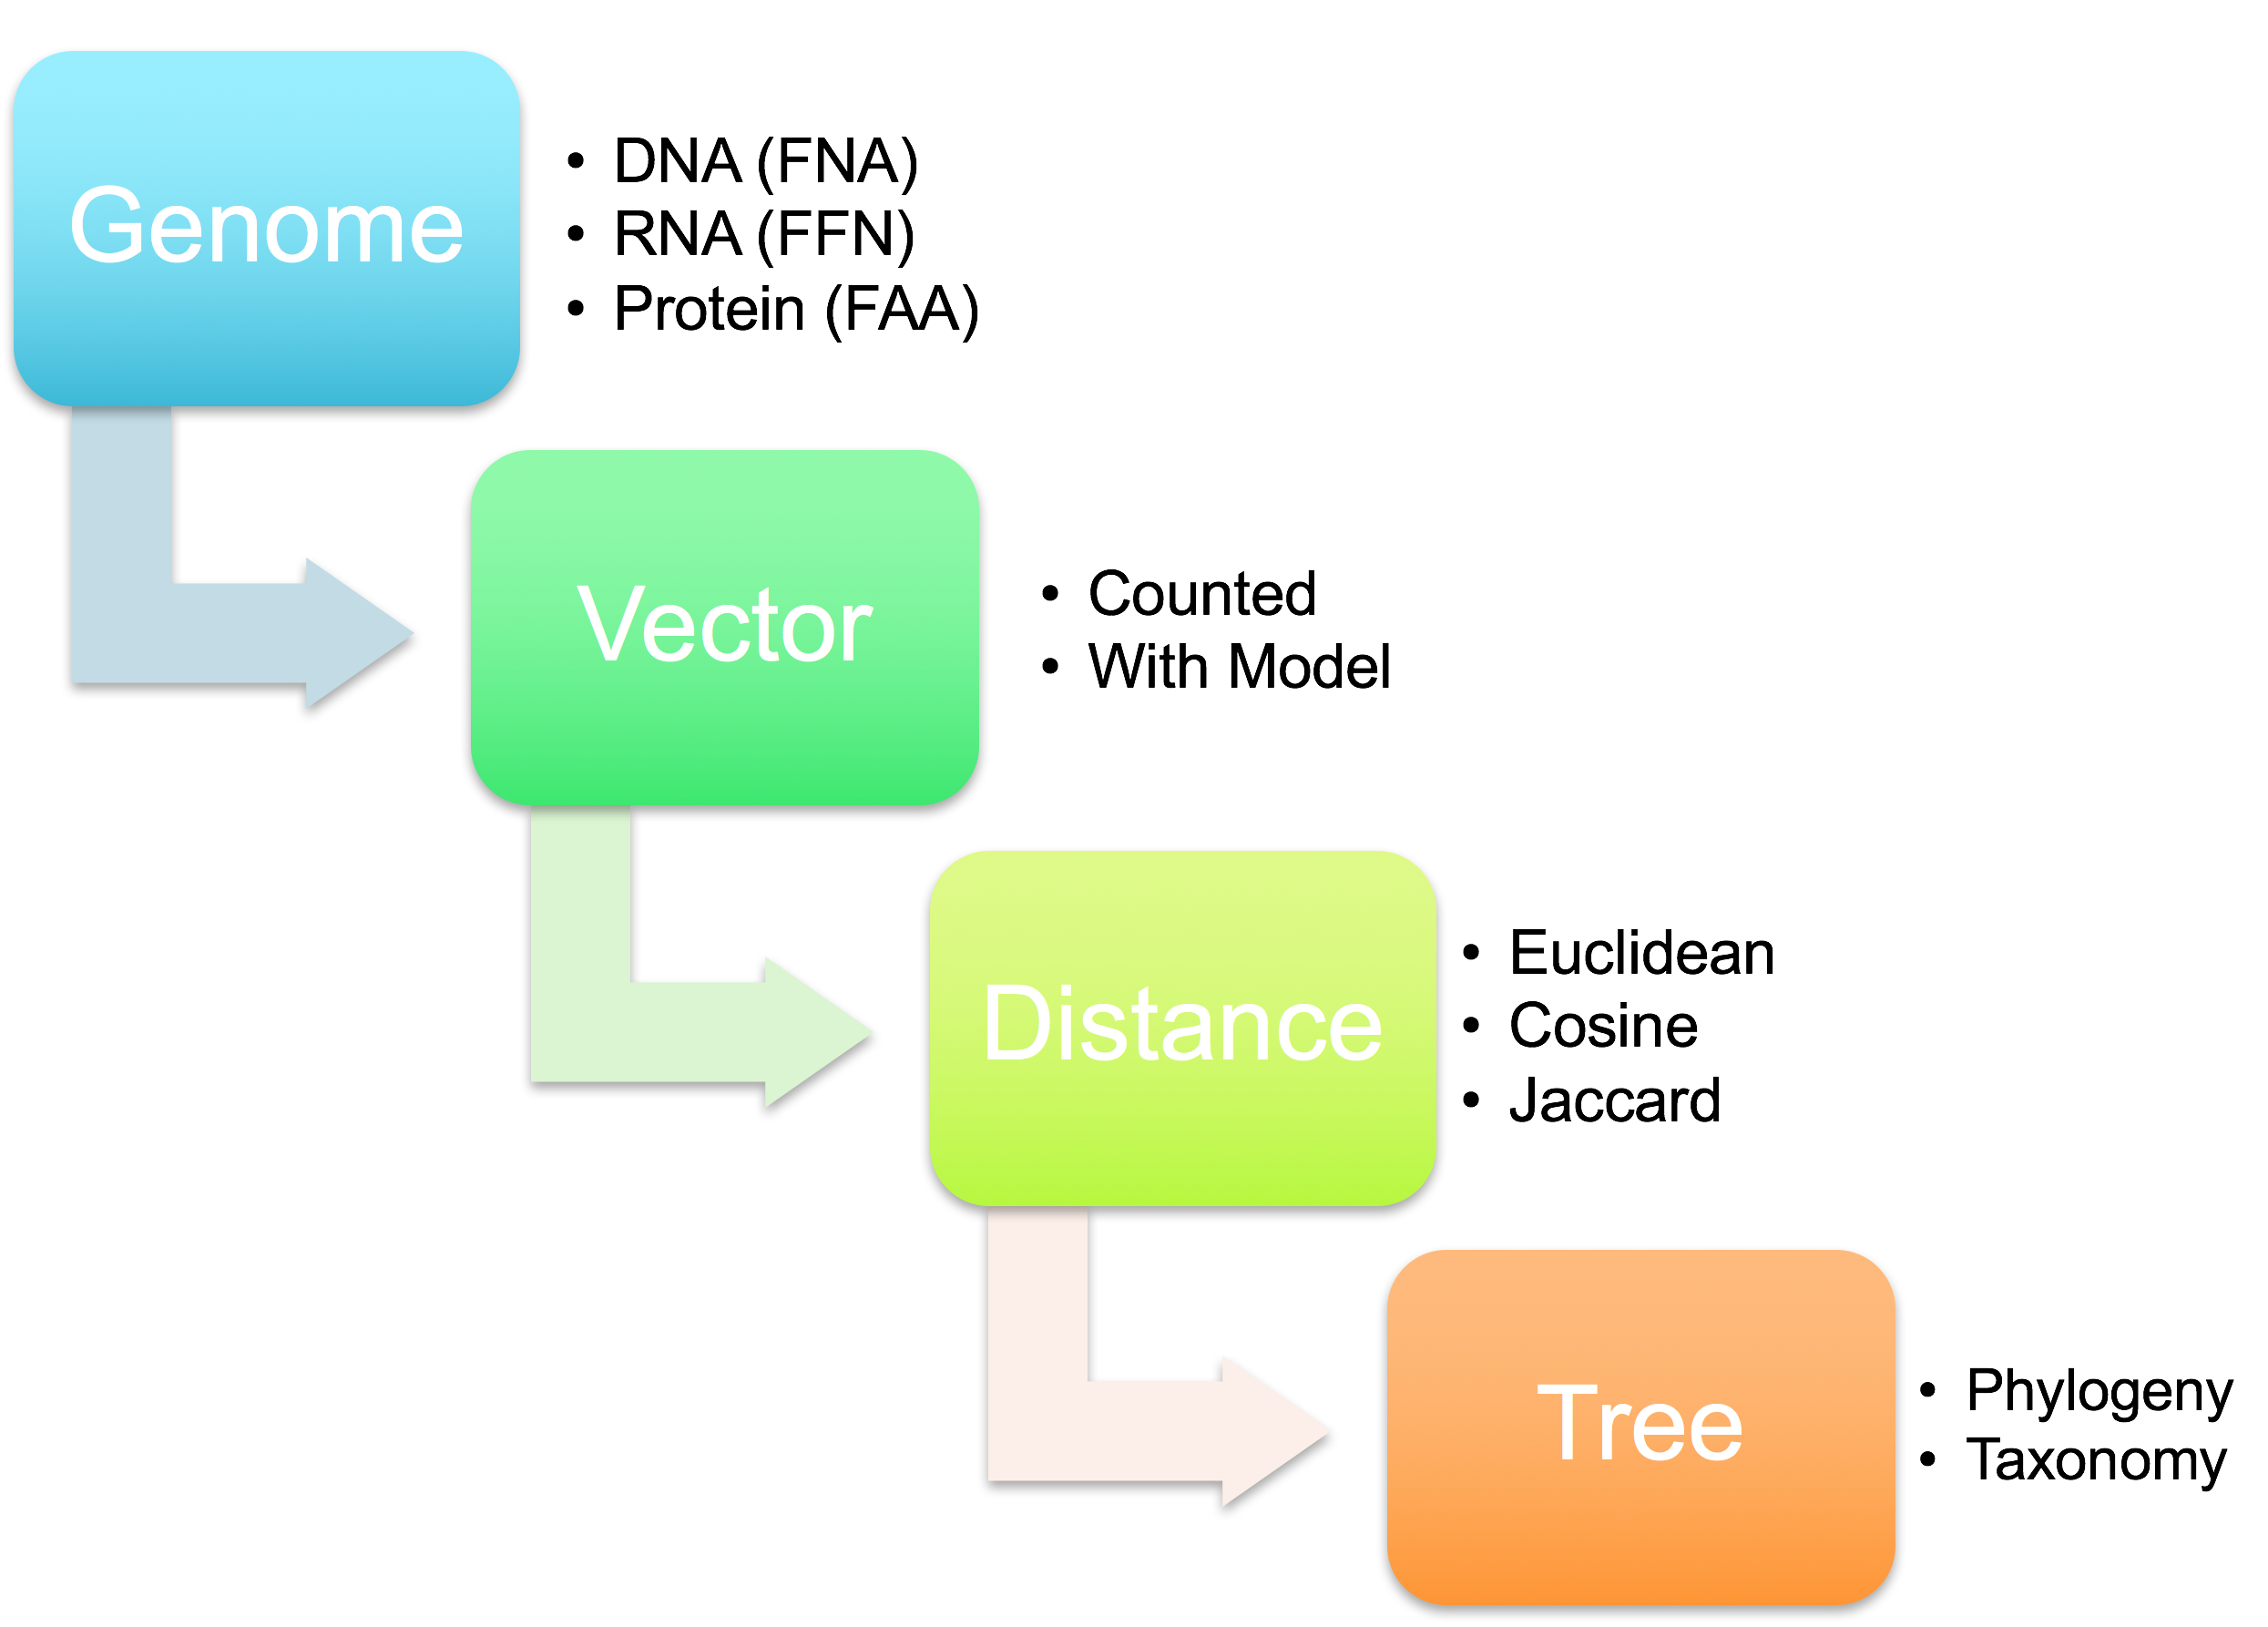
\includegraphics[width=0.8\textwidth]{Scheme.png}
  \caption{The Scheme of CVTree}
\end{figure}

\subsection{Hao Method: The classical CVTree}
The algorithm of CVTree consists of the following steps:
\begin{enumerate}\itemsep 0pt
\item Fix a string length $K$ ($K\in [3,7]$ for Amino Acid sequences and
  $K\in [3,16]$ for nucleotide sequences in 32-bit system). Read in the
  sequence collection of each species separately. Count the number of
  all $K$, $K-1$ and $K-2$ tuples for a species. A {\it raw} Composition
  Vector (CV) of dimension $4^K$ or ${20}^K$ is formed by putting the
  counts of $K$-tuples in lexicographic order.
  \item Calculate the subtraction score for the i-th $K$-tuple:
\begin{equation*}
  a_i(a_1a_2 \cdots a_K) \equiv \frac{f(a_1a_2 \cdots a_K) -
    f^0(a_1a_2 \cdots a_K)}{f^0(a_1a_2 \cdots a_K)}
\end{equation*}
where $f(a_1a_2 \cdots a_K)$ is the frequency of $K$-tuple, $f^0(a_1a_2
\cdots a_K)$ is the frequency predicted from that of $(K-1)$ and $(K-2)$
tuples by using a $(K-2)$-th Markov assumption, \cite{qwh04}.  All
components of the {\it raw} CV is replaced by its subtraction score to
yield a renormalized CV.
\item Using the renormalized CVs to calculate the pairwise dissimilarity
  between two species:
  $$d(A, B)=(1-C(\vec{CV_A},\vec{CV_B}))/2,$$
where
\begin{equation*}
  C(\vec{CV_A},\vec{CV_B})=\frac{\sum_{i=1}^NA_i \times
    B_i}{(\sum_{i=1}^NA_i^2 \times \sum_{i=1}^NB_i^2)^{\frac{1}{2}}}
\end{equation*}

\item Then obtain the phylogenetic tree (Newick Format) based on this
  dissimilarity matrix by Neighbor Joint method.
\end{enumerate}
For more detailed description of the algorithm please consult
\cite{qwh04}. 

\subsection{The update CVTree Algorithm}
There are two new algoriths named by InterSet and InterList. The are based on the 
counted Kstring without the markov model. 

\subsubsection{The InterSet Method} 
\begin{itemize}
  \item From genome to vector: $$v(a_1 a_2 \cdots a_k) = \sigma [f(a_1a_2 \cdots a_k)]$$ 
  where $\sigma = 1$ when $a_1a_2\cdots a_k$ was found in the genome, or $\sigma = 0$.
  \item From vector to distance: for the vector $i$ and $j$, 
  $$D(\vec{v_i},\vec{v_j})= 1 -\sqrt{\frac{\vec{v_i} 
  \cdot \vec{v_j}}{|\vec{v_i}| \cdot |\vec{v_j}}}$$
  \item Then obtain the phylogenetic tree (Newick Format) based on this
  dissimilarity matrix by Neighbor Joint method.
\end{itemize}

\subsubsection{The InterList Method} 
\begin{itemize}
  \item From genome to vector: $$v(a_1a_2\cdots a_k)= f(a_1a_2 \cdots a_k)$$ 
  where $\sigma = 1$ when $a_1a_2\cdots a_k$ was found in the genome, or $\sigma = 0$.
  \item From vector to distance: for the vector $i$ and $j$, 
  $$D(\vec{v_i},\vec{v_j})= 1-\frac{2 \times \sum \min[v_i(a_1a_2\cdots a_k), 
  v_j(a_1a_2\cdots a_k)]}{\sum v_i(a_1a_2\cdots a_k) + \sum v_j(a_1a_2\cdots a_k)}$$
  \item Then obtain the phylogenetic tree (Newick Format) based on this
  dissimilarity matrix by Neighbor Joint method.
\end{itemize}

\section{Version History and Contributors}

Since 2002 the CVTree software has undergone many revisions. A few major
versions were:
\begin{enumerate}\itemsep 0pt
\item Web Server CVTree 1.0 was written by Ji Qi, Hong Luo and Bailin Hao
\item Most 1.x versions of Standalone CVTree was written by Lei Gao;
  Ver. 1.9.6 was written by Ji Qi.
\item Web Server CVTree 2.0 was written by Zhao Xu and Bailin Hao
\item Standalone CVTree 2.4 was written by Zhao Xu
\item Web Server CVTree 3.0 was written by Guanghong Zuo and Bailin Hao
\item Standalone CVTree 3.0 was written by Guanghong Zuo
\item Standalone CVTree 4.0 was written by Guanghong Zuo
\end{enumerate}

\section{Citing CVTree in a Publication}

Please cite:
\begin{enumerate}\itemsep 0pt
\item Ji Qi, Bin Wang, Bailin Hao (2004), Whole proteome prokaryote
  phylogeny without sequence alignment: a K-string composition approach,
  {\it Journal of Molecular Evolution}, {\bf 58}: 1 -- 11.
\item Guanghong Zuo and Bailin Hao (2015) CVTree3 Web Server for 
Whole-genome-based and Alignment-free Prokaryotic Phylogeny and Taxonomy.
\newblock {\em Genomics Proteomics Bioinformatics, } {\bf 13}: 321--331.
\end{enumerate}

\begin{thebibliography}{}
\bibitem[Qi {\em et~al.}, 2004{\em{a}}]{qlh04}
Qi,J., Luo,H.  and Hao,B. (2004{\em{a}}) Cvtree: a phylogenetic tree
  reconstruction tool based on whole genomes.
\newblock {\em Nucleic acids research, } {\bf 32}, W45--7.
\newblock PMID: 15215347.

\bibitem[Qi {\em et~al.}, 2004{\em{b}}]{qwh04}
Qi,J., Wang,B.  and Hao,B. (2004{\em{b}}) Whole proteome prokaryote phylogeny
  without sequence alignment: a k-string composition approach.
\newblock {\em Journal of Molecular Evolution, } {\bf 58}, 1--11.

\bibitem[Xu and Hao, 2009]{xh09}
Xu,Z. and Hao,B. (2009{\em{}}) Cvtree update: a newly designed phylogenetic
  study platform using composition vectors and whole genomes.
\newblock {\em Nucleic Acids Research, } {\bf 37 Web Server Issue}, W174--W178.
\bibitem[Zuo and Hao, 2015]{zh15}
Zuo,G. and Hao,B. (2015{\em{}}) CVTree3 Web Server for Whole-genome-based and Alignment-free Prokaryotic Phylogeny and Taxonomy.
\newblock {\em Genomics Proteomics Bioinformatics, } {\bf 13}, 321--331.
\end{thebibliography}
\end{document}
